\section[Ottimizzazione]{Problemi di ottimizzazione e algoritmi greedy}
\subsubsection{Grafi pesati}
Sono grafi in cui associo delle informazioni agli archi o ai nodi.\\
$G = (V, E)$ grafo,\\
$w: E \rightarrow \mathbb{R}$ funzione peso.\\
Alcuni esempi di problemi che utilizzano i grafi pesati sono:
\begin{itemize}
    \item Cammini minimi
    \item Commesso viaggiatore
    \item Albero ricoprente minimo
\end{itemize}

\subsubsection{Problemi di ottimizzazione}
Tra tutte le soluzioni \emph{ammissibili} per un problema voglio determinarne una 
\emph{ottima} rispetto ad un dato criterio.

\subsubsection{Tecnica greedy}
$P$ = problema di ottimizzazione
$C$ = insieme di candidati
Voglio trovare $S^{*} \subseteq C$ ottima.
\begin{itemize}
    \item In una sequenza di passi costruisco, a partire dall'insieme vuoto, una soluzione ammissibile $S \subseteq C$
    \item Ad ogni passo si espande una soluzione parziale già ottenuta
    \item L'algoritmo termina quando non è più possibile espandere la soluzione parziale
\end{itemize}

\noindent L'espansione della soluzione può essere vista in questo modo:
\begin{itemize}
    \item \textbf{Soluzione ammissibile}\\
    La soluzione parziale soddisfa i vincoli del problema
    \item \textbf{Scelta dell'ottimo locale}\\
    Tra i candidati disponibili si sceglie quello che, al momento, appare migliore 
    \item \textbf{Scelta irrevocabile}\\
    Le scelte effettuate non vengono più messe in discussione
\end{itemize}

\begin{algorithm}
    \caption{Schema tecnica greedy}
    \Indm\textbf{Algoritmo} \emph{greedy(insieme C)} $\rightarrow$ \emph{soluzione} \\
    \Indp$S \leftarrow \emptyset$\\
    \While{$C \neq \emptyset$}{
        $x \leftarrow seleziona(C)$  \texttt{/* elemento considerato "migliore" al momento */}\\
        $C \leftarrow C - \lbrace x \rbrace$\\
        \If{$S \cup \lbrace x \rbrace$ è ammissibile}{
            $S \leftarrow S \cup \lbrace x \rbrace$
        }
    }
    \Return{$S$}
\end{algorithm}
\clearpage

\subsubsection{Programmazione dinamica}
Si tratta di un approccio bottom-up. A differenza del divide-et-impera i sottoproblemi vengono 
risolti prima e le soluzioni parziali vengono salvate.
Vediamo alcuni esempi.\\
\textbf{Esempio 1}: Dato un vettore $V$ di interi in $\mathbb{Z}$ trovare un sottovettore di somma massima.\\
$V[1...n]$ vettore in input\\
Sottovettore con
\begin{itemize}
    \item Indice di inizio $i$ con $1 \le i \le n$
    \item Indice di fine $f$ con $1 \le f \le n$
\end{itemize}
\begin{algorithm}
    \caption{Sottovettore di somma massima}
    \Indm\textbf{Algoritmo} \emph{sottovettoreMax(Array V[1...n])} $\rightarrow$ \emph{intero, intero}\\
    \Indp$max \leftarrow V[1], \space inizio \leftarrow 1, \space fine \leftarrow 1$\\
    \For{$f \leftarrow 1$ \textbf{to} $n$}{
        $somma \leftarrow$ somma di $V[1...f]$\\
        \If{$somma > max$}{
            $max \leftarrow somma$ \\
            $inizio \leftarrow i$\\
            $fine \leftarrow f$
        }
    }
    \Return{($inizio, \space fine$)}
\end{algorithm}

\textbf{Esempio 2}: trovare il cammino di valore minimo in una matrice $n \cdot n$\\
$C[i,j]$ = costo cammino minimo che inizia nella colonna 1 e termina nella posizione ($i, j$)\\
La prima colonna è uguale alla prima colonna della matrice di partenza.\\
Per le altre colonne $C[i, j] = M[i,j] + min\lbrace C[i-1, j-1], C[i, j-1], C[i+1, j-1]\rbrace$\\
Anche se mi fermo prima di risolvere il problema ho comunque una soluzione ottima per il
sottoproblema.
\begin{algorithm}
    \caption{Cammino minimo in una matrice}
    \Indm\textbf{Algoritmo} \emph{camminoMinimo(Matrice M[1...n, 1...n])} $\rightarrow$ \emph{intero}\\
    \Indp Sia $C[1...n, 1...n]$ una matrice\\
    \For{$i \leftarrow 1$ \textbf{to} $n$}{
        $C[i, 1] = M[i, 1]$ \texttt{/* riempio la prima colonna */}
    }
    \For{$j \leftarrow 2$ \textbf{to} $n$}{
        \For{$i \leftarrow 1$ \textbf{to} $n$}{
            $min \leftarrow C[i, j-1]$\\
            \If{$i > 1$ \textbf{and} $C[i-1, j-1] < min$}{
                $min \leftarrow C[i-1, j-1]$
            }
            \If{$i < n$ \textbf{and} $C[i+1, j-1] < min$}{
                $min \leftarrow C[i+1, j-1]$
            }
            
        }
    }
    $C[i,j] = M[i,j] + min$\\
    \For{$i \leftarrow 2$ \textbf{to} $n$}{
        \If{$C[i, n] < min$}{
            $min \leftarrow C[i, n]$
        }
    }
    \Return{min}
\end{algorithm}

\clearpage


\subsection{Albero ricoprente minimo}
Ricordiamo che dato un grafo non orientato e pesato, un \emph{albero ricoprente minimo} del grafo è un albero ricoprente
il cui peso sia minimo tra tutti gli alberi ricoprenti del grafo.
\begin{figure}[h]
    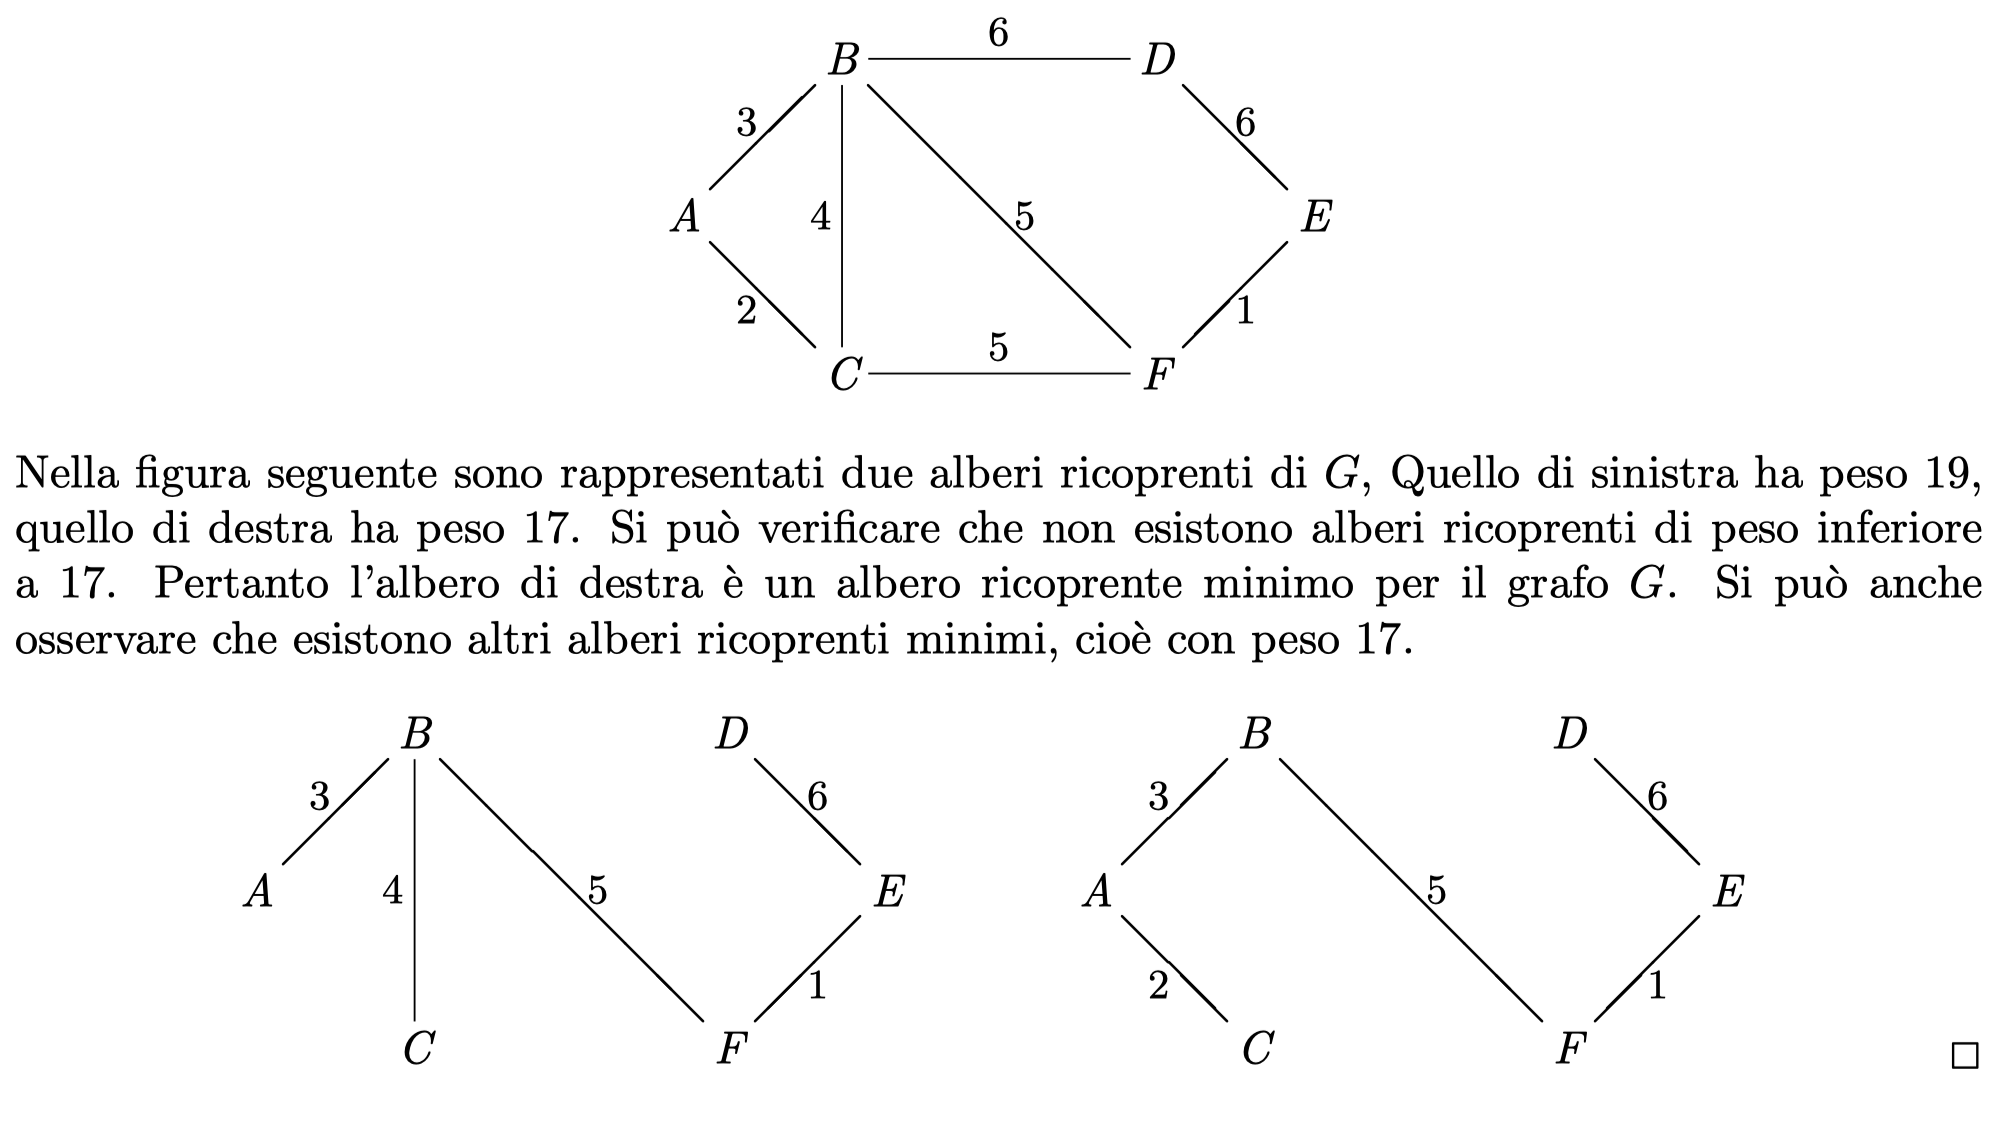
\includegraphics[width=\textwidth]{albero_ricoprente_minimo.png}
\end{figure}
Vediamo ora due algoritmi per trovare un albero ricoprente minimo di un grafo connesso, non orientato
e pesato. In entrambi gli algoritmi viene costruito in modo incrementale utilizzando una strategia greedy.
\clearpage
\subsubsection{Algoritmo di Kruskal}
Il primo algoritmo risolve il problema costruendo un grafo $T$ che ha gli stessi 
vertici di $G$ e, inizialmente, è privo di archi. L'algoritmo esamina $G$
in ordine di peso non decrescente. Un arco viene aggiunto a $T$ se, insieme a 
quelli già scelti, non forma cicli, altrimenti viene scartato e non sarà più considerato.
Pertanto, ad ogni passo, il grafo $T$ è una foresta di alberi. Ogni volta che si aggiunge un arco
si connettono tra loro due alberi della foresta che diventano, con l'arco aggiunto, un unico albero.
Alla fine, quando sono stati esaminati tutti gli archi, $T$ è un unico albero ricoprente che, come dimostreremo, è di peso minimo per il grafo 
$G$ dato.
Si può dimostrare che l'algoritmo trova sempre la soluzione ottima, cioè trova sempre un albero ricoprente di peso minimo.\\
\begin{figure}[h]
    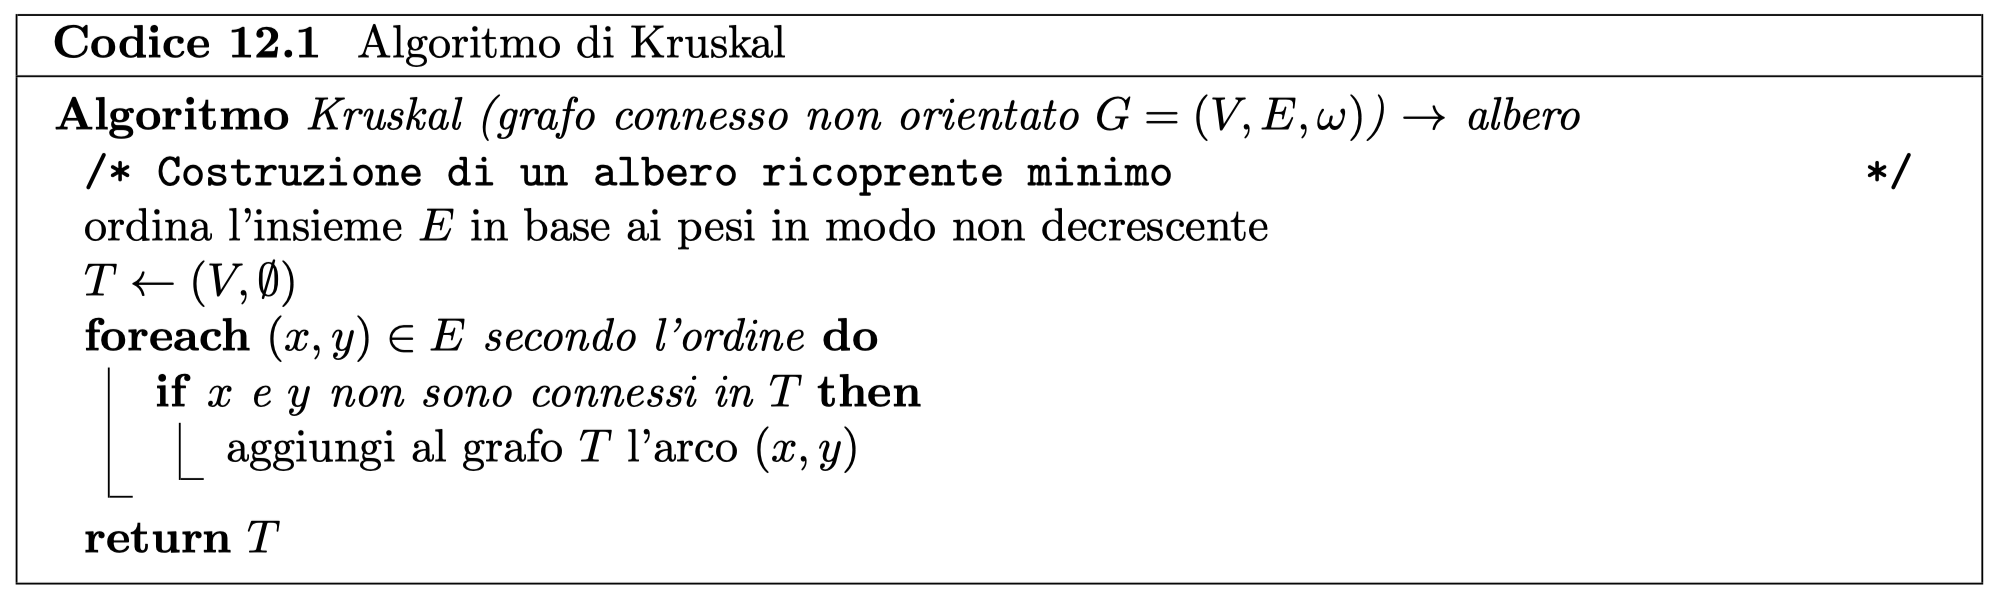
\includegraphics[width=\textwidth]{kruscal.png}
\end{figure}
Studiamo ora una possibile implementazione dell'algoritmo di Kruskal. È utile rappresentare 
il grafo come lista di archi. La lista può essere rappresentata direttamente in un array, sul quale applicare uno degli algoritmi di ordinamento (in base ai pesi degli archi).
Insieme al grafo $T$ che viene costruito, utilizziamo una struttura che permetta, quando si ispeziona 
un arco $(x, y)$, di decidere facilmente se i vertici $x$ e $y$ sono già connessi in $T$.
A tale scopo possiamo considerare partizioni dell'insieme dei vertici $V$, in cui due vertici appartengono
allo stesso elemento della partizione se e solo se sono connessi in $T$. In altre 
parole ogni elemento della partizione rappresenta una componente connessa di $T$.
\begin{itemize}
    \item Inizialmente ogni vertice di $V$ costituisce un singolo insieme della partizione (T non contiene archi e dunque non ci sono archi connessi tra loro).
    \item Quando esaminiamo un arco ci sono due possibilità:
    \begin{itemize}
        \item Se $x$ e $y$ appartengono allo stesso elemento della partizione significa 
        che sono già connessi in $T$. In tal caso l'arco $(x,y)$ non viene aggiunto a $T$ perchè creerebbe un ciclo
        \item Se $x$ e $y$ appartengono ad elementi diversi della partizione allora non sono connessi:
        aggiungendo l'arco $(x,y)$ a $T$ rendiamo ciascun vertice dell'elemento a cui appartiene $x$ connesso con ciascun vertice dell'elemento a cui appartiene $y$,
        cioè rendiamo le due componenti connesse a cui appartengono $x$ e $y$ un'unica componente connessa.
    \end{itemize}
\end{itemize}
\noindent La partizione può essere rappresentata mediante le strutture Union-Find. Per 
verificare se $x$ e $y$ appartengono allo stesso insieme della partizione confronto i risultati di 
\texttt{FIND(x)} e \texttt{FIND(y)}. Per unire due elementi della partizione utilizziamo \texttt{UNION}.\\
Stimiamo ora il tempo di calcolo in funzione del numero $n$ di vertici e $m$ di archi del grafo $G$ in input.
Assumendo il criterio di costo uniforme, supponiamo che i confronti tra i pesi degli archi avvengano in tempo costante. Dobbiamo tenere conto dei seguenti tempi:
\begin{itemize}
    \item Ordinamento di $E$:\\
    Utilizziamo \texttt{heapSort} e ordiniamo in tempo $O(m \log m)$
    \item Operazioni Union/Find:\\
    Supponiamo di usare QuickUnion con bilanciamento in altezza in cui ciascuna
    operazione \texttt{MAKESET} viene effettuata in tempo costante, \texttt{FIND} in tempo $O(\log n)$
    e \texttt{UNION} in tempo costante, dove $n$ è il numero di elementi presenti
    complessivamente negli insiemi della partizione. L'algoritmo effettua queste operazioni:
    \begin{itemize}
        \item $n$ operazioni di \texttt{MAKESET}: tempo $O(n)$
        \item $2m$ operazioni di \texttt{FIND}: tempo $O(m \log n)$
        \item $n - 1$ operazioni di \texttt{UNION}: tempo $O(n)$
    \end{itemize}
\end{itemize}

\noindent Sommando i vari tempi otteniamo $O(m \log n)$ approssimabile a $O(m \log m)$.
Se i pesi sono interi si potrebbe ridurre il costo dell'ordinamento usando \texttt{radixSort}.
\begin{figure}[h]
    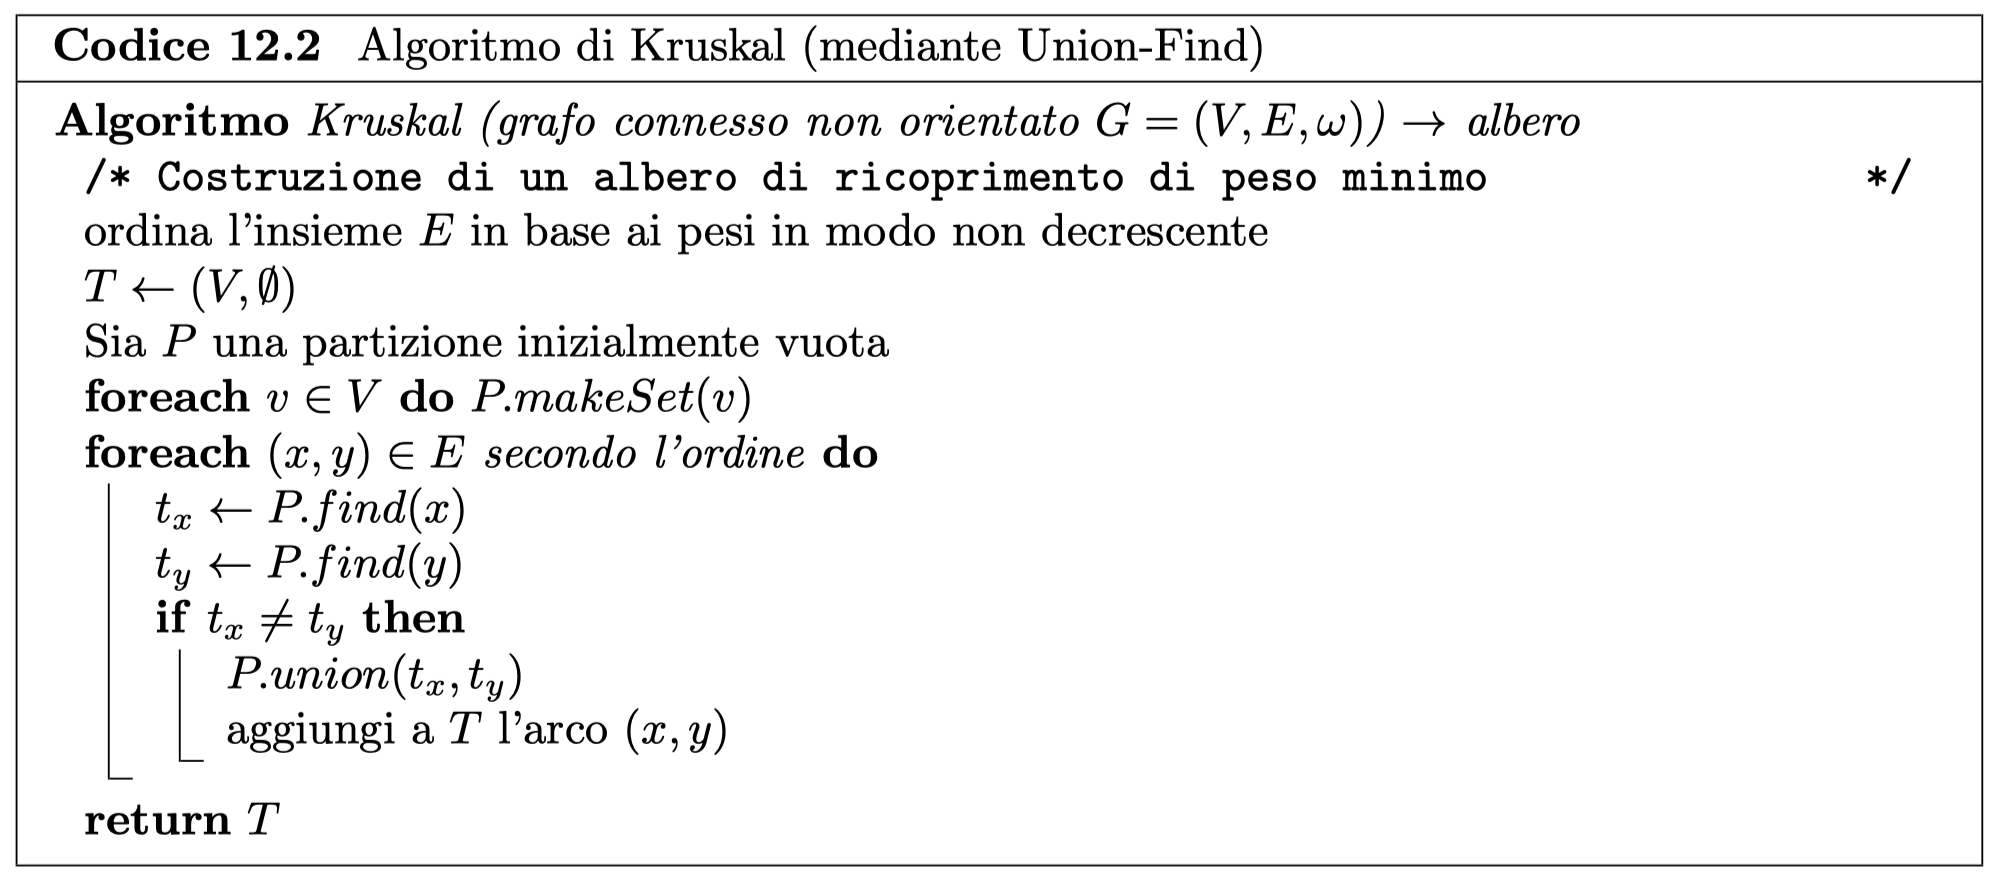
\includegraphics[width=\textwidth]{kruscal_union_find.png}
\end{figure}
\clearpage

\subsubsection{Algoritmo di Prim}
Dato in ingresso un grafo connesso, non orientato con pesi sugli archi, l'algoritmo inizia
costruendo un albero $T$ formato da un unico vertice $s$ qualsiasi del grafo.
Ad ogni passo l'albero $T$ viene espanso scegliendo tra tutti gli archi che hanno un vertice in $T$ e l'altro non in $T$, un arco
di peso minimo. Tale arco viene aggiunto a $T$ (insieme al vertice che non era in $T$). Si può dimostrare che, come l'algoritmo di 
Kruskal, anche questo trova sempre una soluzione ottima.\\
\begin{figure}[h]
    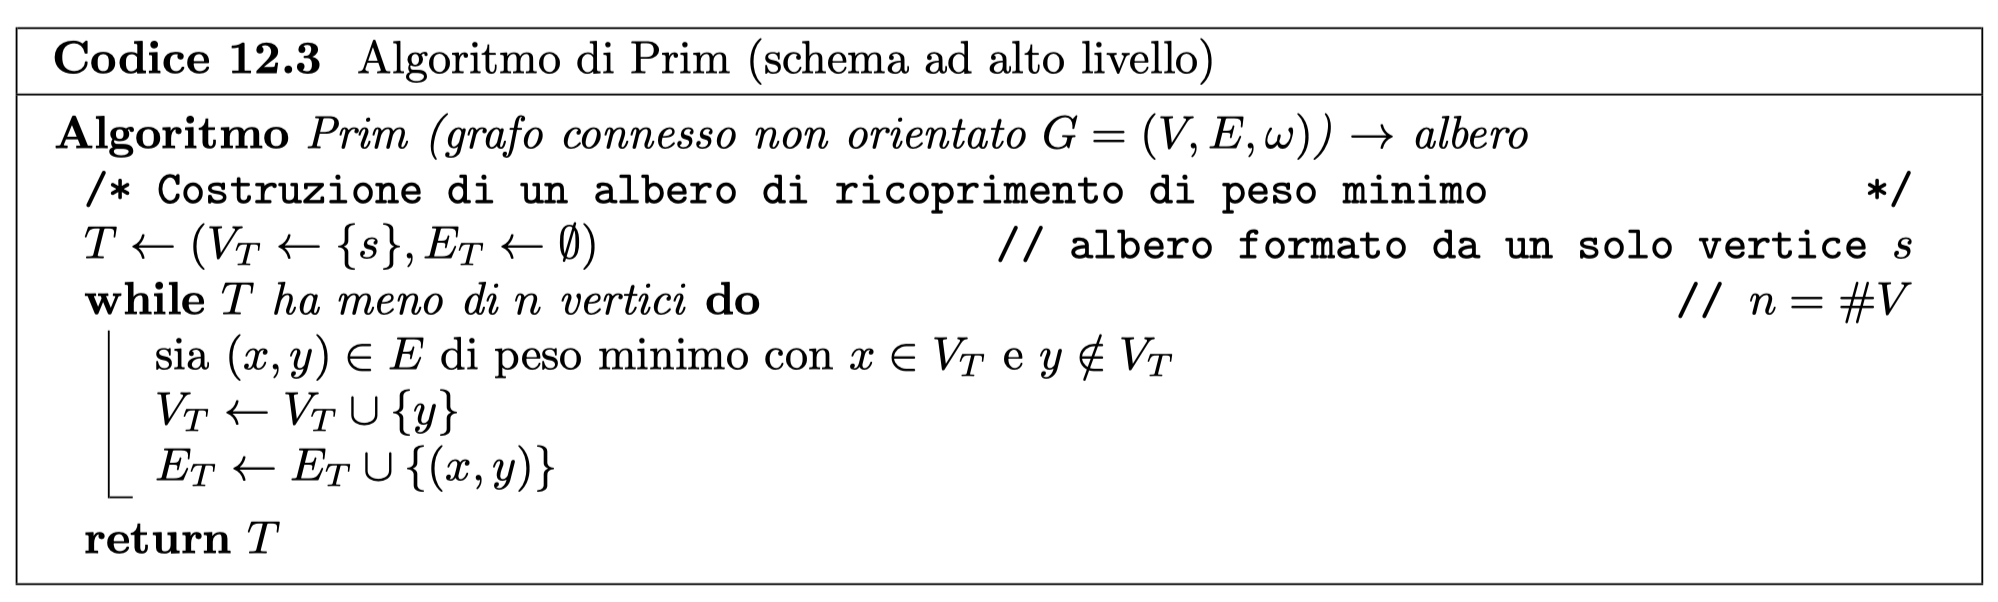
\includegraphics[width=\textwidth]{prim_alto_livello.png}
\end{figure}
L'algoritmo di Prim può essere implementato ricorrendo ad una coda con priorità $C$, contenente 
un elemento per ogni vertice che deve ancora essere inserito nell'albero, secondo 
la tecnica che descriviamo ora:
\begin{itemize}
    \item Ad ogni passo, per ogni vertice $v$ non ancora in $T$ consideriamo le seguenti informazioni:
    \begin{itemize}
        \item $d[v]$: minimo peso di un arco tra un vertice appartenente all'albero $T$
        già costruito e $v$, 
        \item $vicino[v]$: un vertice $u$ nell'albero $T$ già costruito con distanza minima da $v$
    \end{itemize}
    \item La coda con priorità $C$ contiene ciascun vertice $v$ non ancora inserito in $T$ con priorità $d[v]$
    \item Inizialmente l'albero è vuoto. Pertanto, per ogni vertice $v$, si pone 
    $d[v] = \infty$, mentre il valore di $vicino[v]$ non è definito. Ogni vertice viene inserito in $C$
    \item Ad ogni passo si sceglie un vertice $y$ corrispondente al minimo in $C$. (Al primo passo se ne sceglie uno qualsiasi)
    \item Nei passi successivi al primo si considera il "vicino" $x$ in $T$ del vertice $y$ scelto.
    L'arco $(x,y)$ è pertanto un arco di peso minimo con un vertice $x$ in $T$ e l'altro vertice $y$ non in $T$.
    Il vertice $y$ e l'arco $(x,y)$ vengono aggiunti all'albero.
    \item Si ricalcolano le priorità dei vertici, tenendo conto del nuovo vertice $y$
    inserito in $T$. Per ogni arco $(y,z)$ uscente da $y$ con $z$ non in $T$, nel caso 
    il peso $w(y,z)$ risulti minore di $d[z]$, si modifica $d[z]$ e si aggiorna la coda con priorità e l'informazione relativa al vicino di $z$.
    \item Queste operazioni vengono ripetute fino a svuotare la coda. A quel punto si può restituire $T$
\end{itemize}
\clearpage

\subsubsection*{Tempo di calcolo}
Prima di tutto assumiamo che il grafo in ingresso sia rappresentato mediante liste di adiacenza o di incidenza. Questo 
permette di trovare facilmente tutti gli archi entranti incidenti su un vertice. 
La coda con priorità può essere rappresentata come un array di $n$ elementi 
e riempita in $O(n)$. Verranno eseguite in totale $n$ operazioni \texttt{deleteMin()}, ciascuna delle
quali impiega tempo al più $O(\log n)$, per un tempo complessivo pari a $O(n \log n)$.
Anche tempo complessivo utilizzato dalle operazioni \texttt{changeKey} è $O(m \log n)$.
Sommando questi tempi otteniamo $O(m \log n)$, come per Kruskal. Con una implementazione
basata sugli \emph{heap di Fibonacci} è possibile ottenere tempo $O(m + n \log n)$ che è meglio del precedente 
in quanto il numero di archi nel grafo è alto.
\begin{figure}[h]
    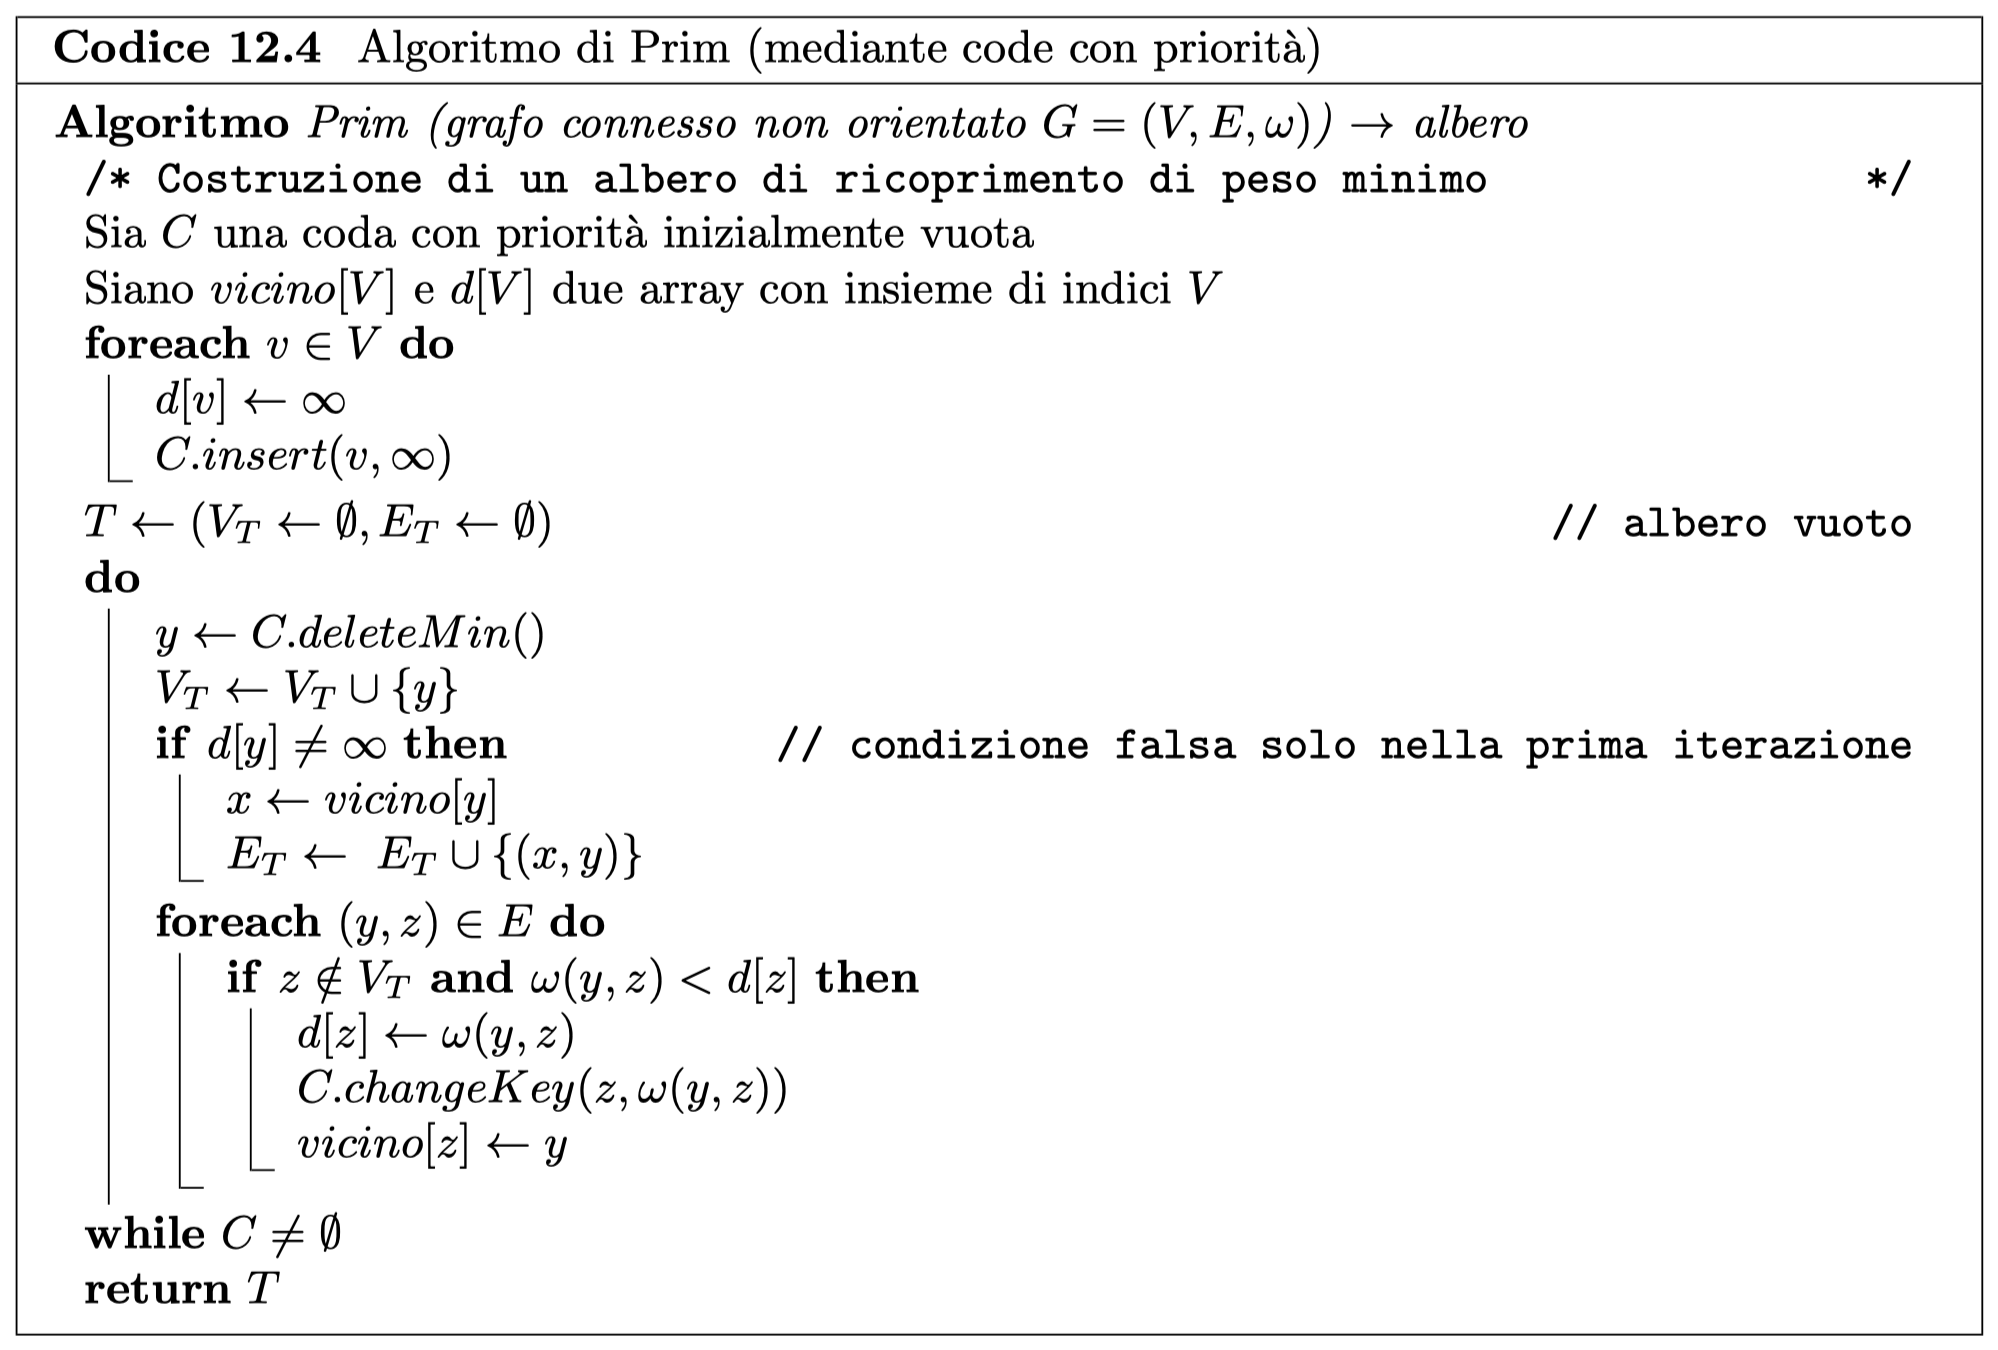
\includegraphics[width=\textwidth]{prim_1.png}
\end{figure}
\begin{figure}[h]
    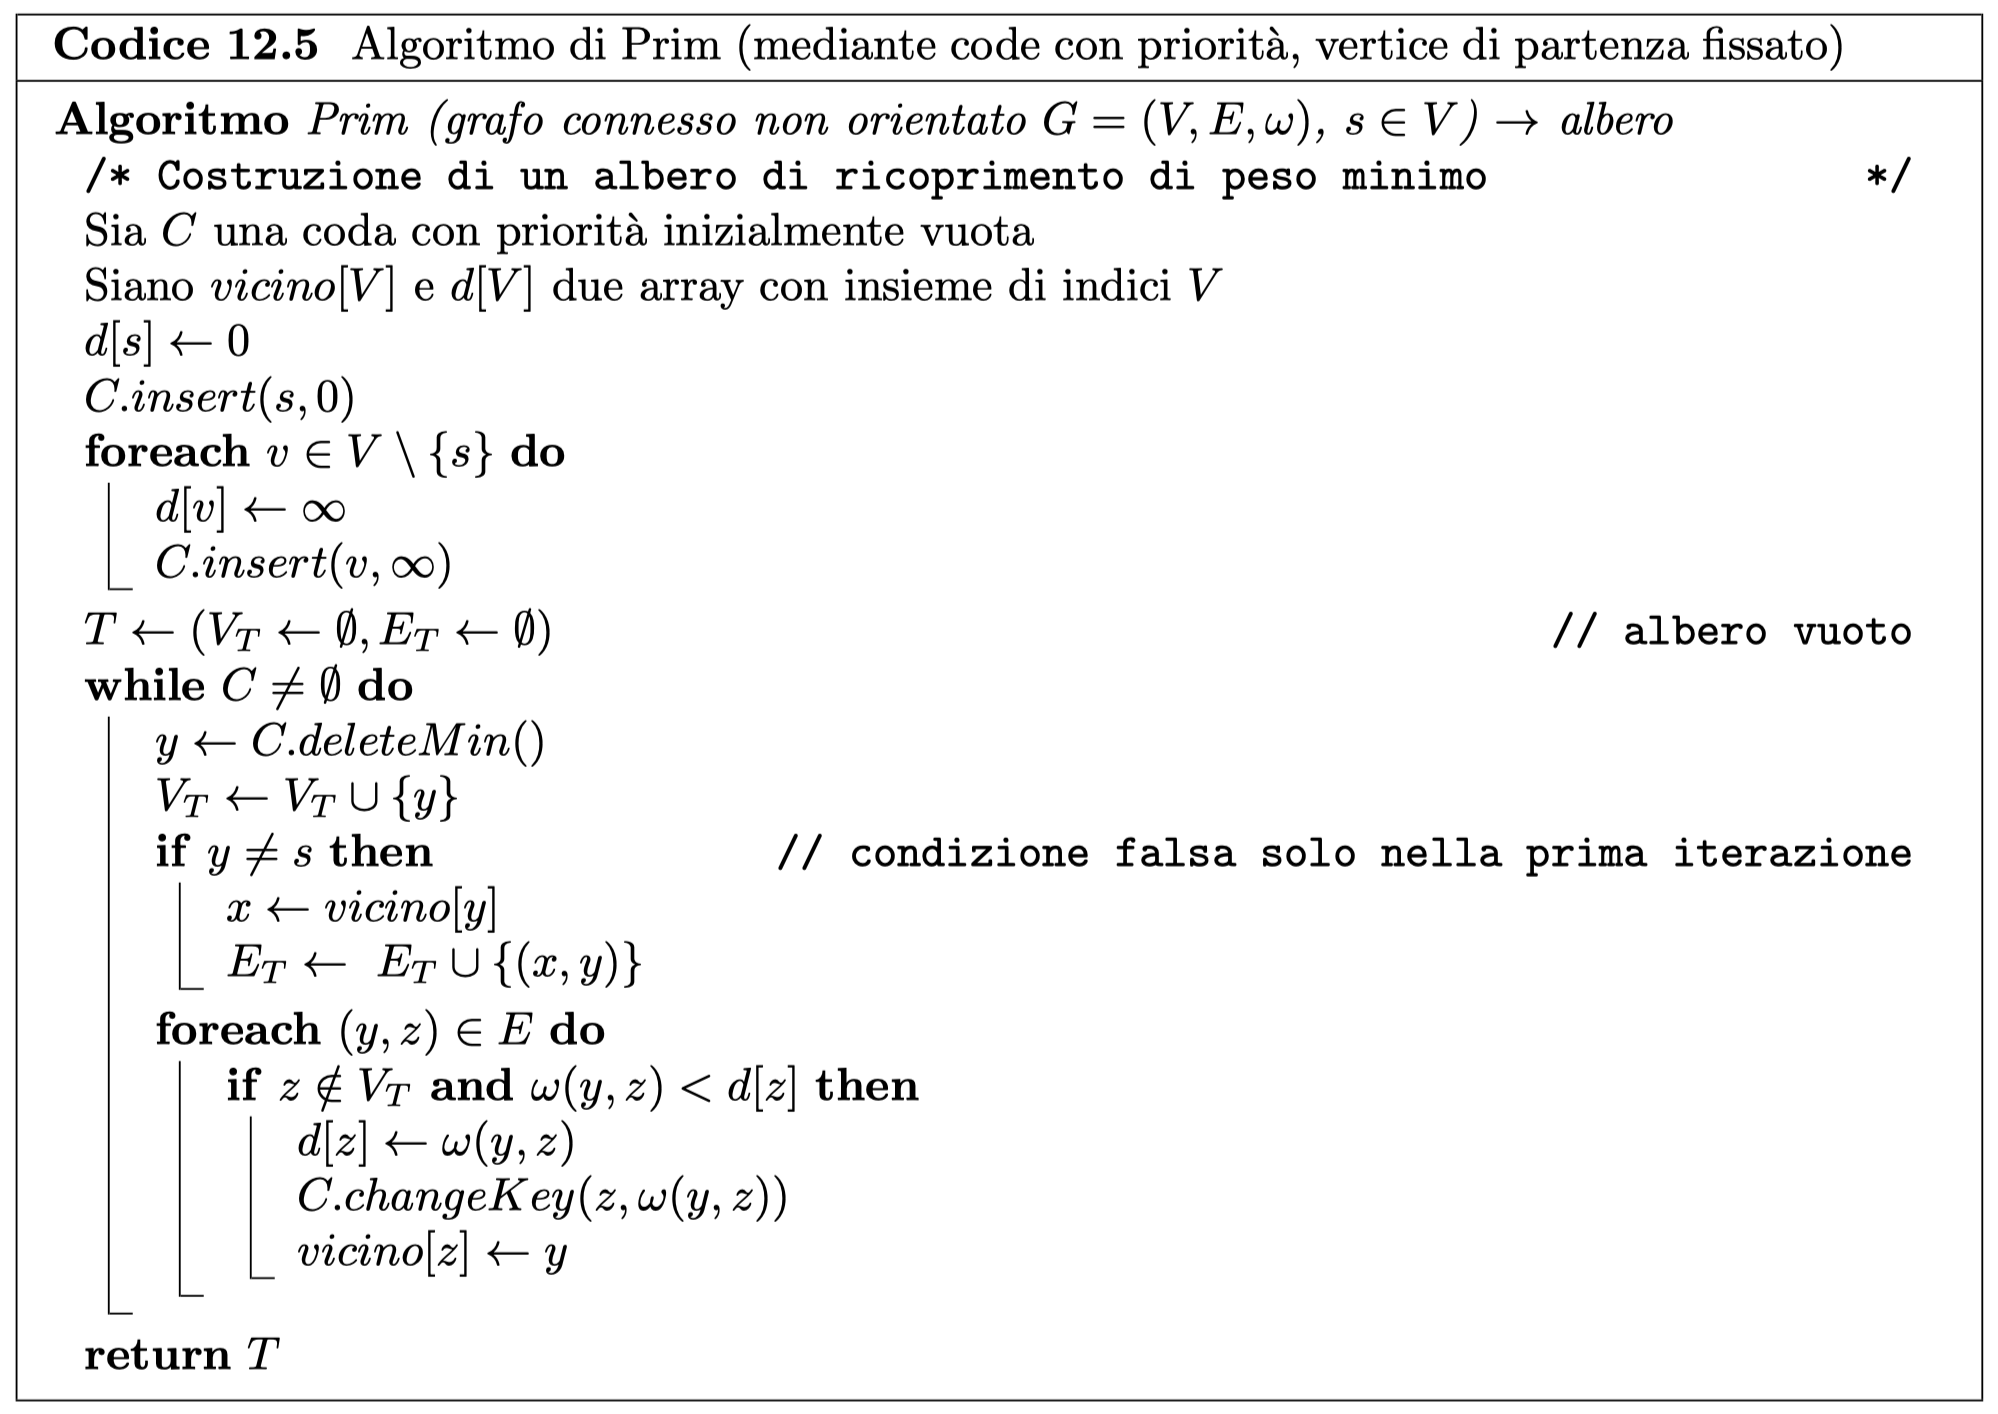
\includegraphics[width=\textwidth]{prim_2.png}
\end{figure}
\clearpage

\subsection{Cammini minimi}
Siano:
\begin{itemize}
    \item $G(V, E)$ un grafo orientato
    \item $w$ funzione peso
    \item $\pi = <V_0...V_k>$ un cammino da $V_0$ a $V_k$
    \item $w(\pi)$ peso del cammino
\end{itemize}

Un cammino minimo tra due vertici è il cammino che ha peso minore tra tutti i cammini tra i due vertici.\\
Alcune proprietà dei cammini minimi:
\begin{enumerate}
    \item Se $\pi$ è un cammino minimo tra $x$ e $y$ che passa per un vertice $v$ allora:
    \begin{itemize}
        \item La parte da $x$ a $v$ è un cammino minimo 
        \item La parte da $v$ a $y$ è un cammino minimo 
    \end{itemize}
    \item Se tutti i pesi sono positivi allora ogni cammino minimo è semplice
    \item Se ci sono pesi negativi ma non ci sono cicli di peso negativo allora 
    tra ogni coppia di vertici esiste un cammino minimo semplice
\end{enumerate}
Per rappresentare grafi pesati posso usare liste di adiacenza con associate ad ogni arco le informazioni riguardanti il peso,
oppure una matrice dei pesi in cui se tra due vertici c'è un arco scrivo il suo peso, altrimenti scrivo $\infty$.
\clearpage
\subsubsection{Algoritmo di Floyd-Warshall}
Questo algoritmo calcola le lunghezze dei cammini minimi tra ogni coppia di vertici.\\
Gli elementi $d_{ij}$ sono uguali a:
$\begin{cases}
    w(V_i, V_j) & \text{se} \space (V_i, V_j) \in E \space \text{e} V_i \neq V_j\\
    0 & \text{se} \space V_i = V_j\\
    \infty & \text{altrimenti}
\end{cases}$
Lavora correttamente anche con pesi negativi purchè non ci siano cicli negativi.
\\
\begin{figure}[h]
    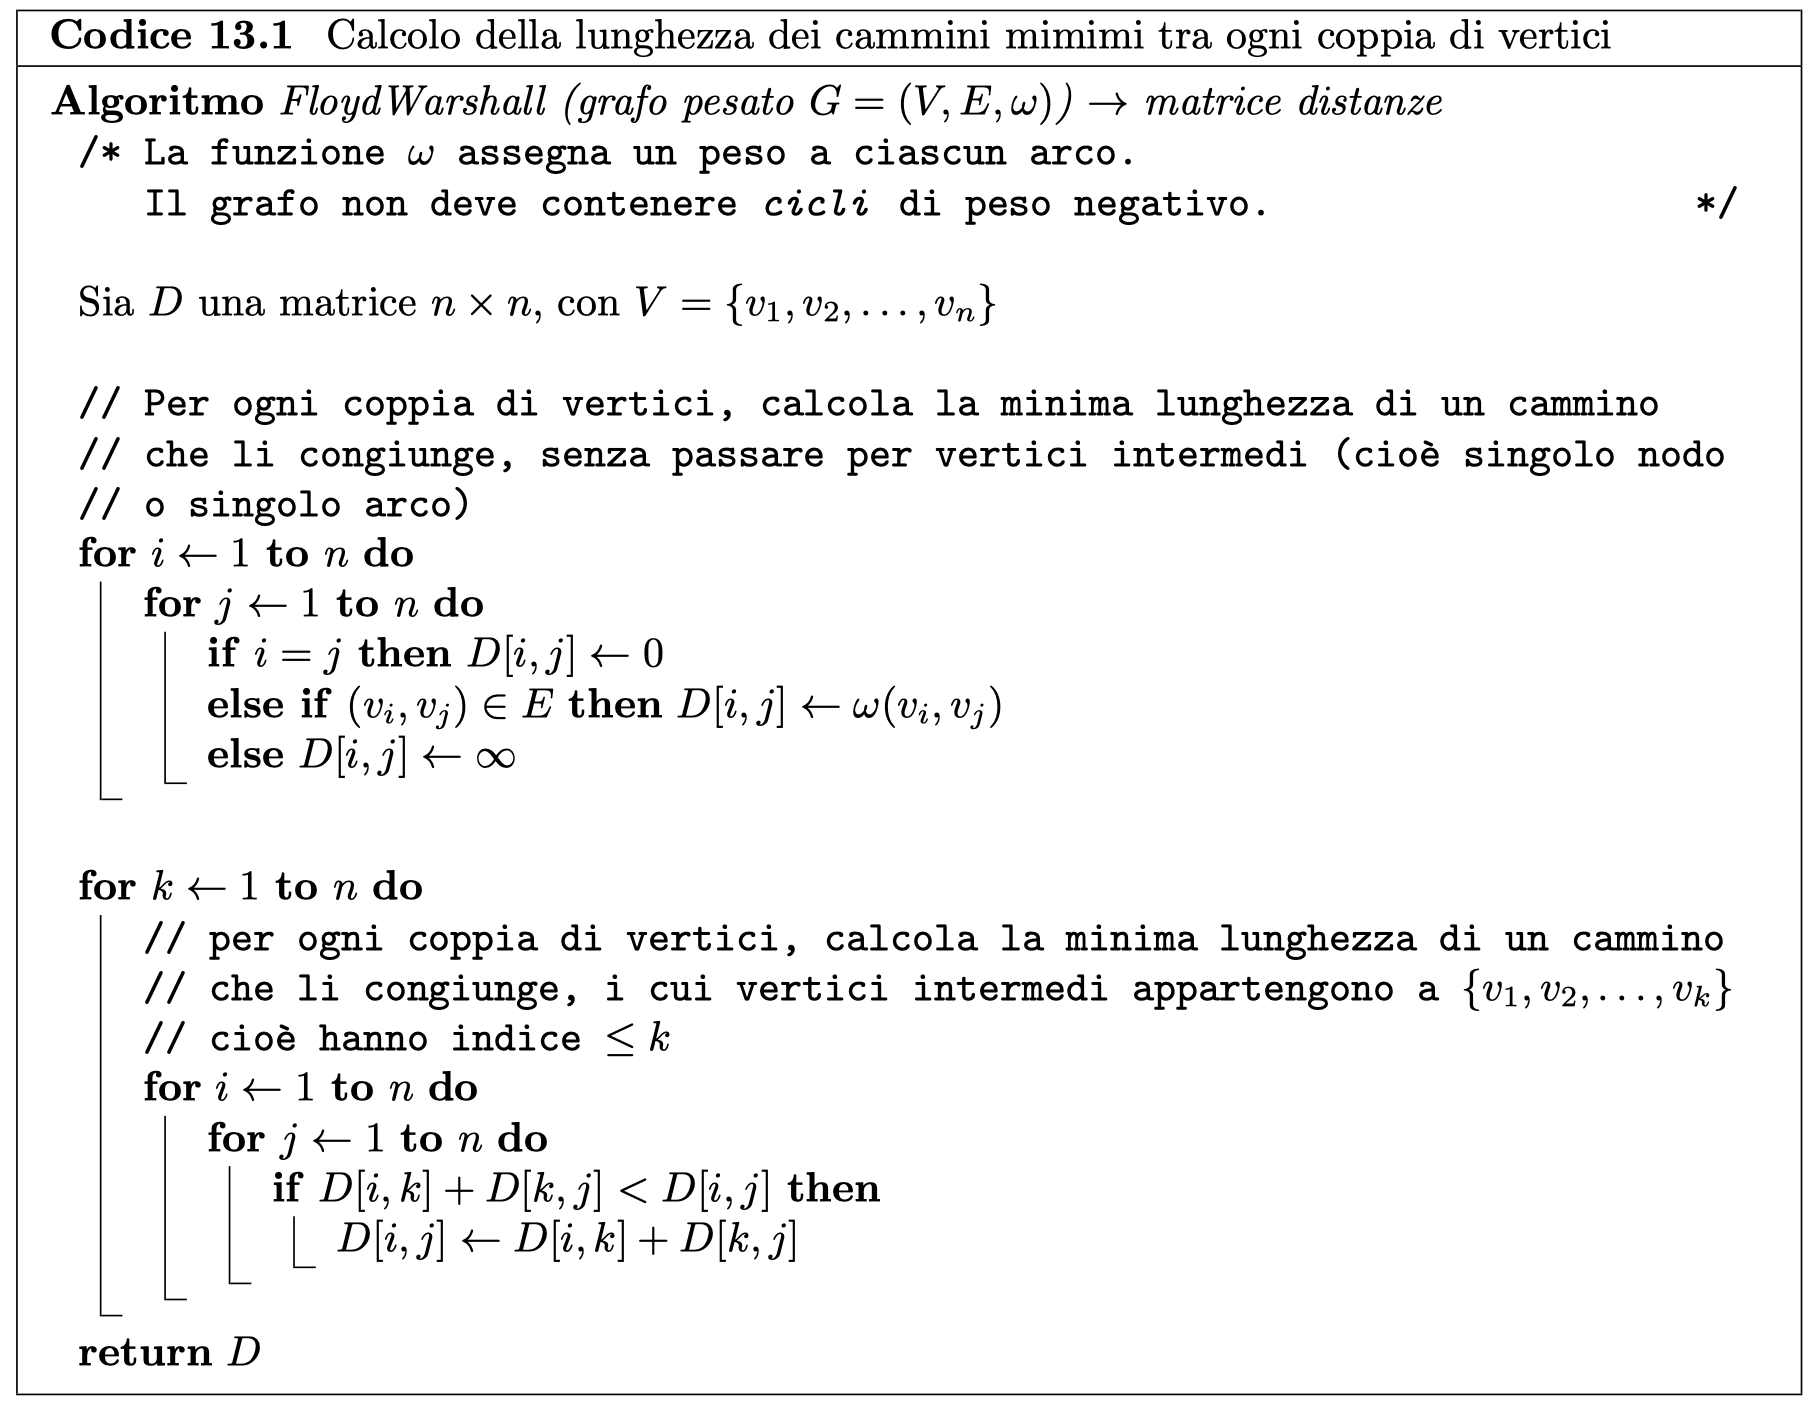
\includegraphics[width=\textwidth]{floydwarshall_1.png}
\end{figure}
\\Esiste anche un'altra versione in cui viene calcolata anche una matrice $P$ che può essere utilizzata per ricavare i cammini minimi.
Dopo l'iterazione $k$, l'elemento $D[i,j]$ contiene la lunghezza del cammino minimo i cui vertici intermedi hanno indice al più $k$.
L'elemento $P[i,j]$ contiene il massimo indice di tali vertici intermedi.
Pertanto, se alla fine dell'esecuzione $P[i,j]$ è 0, significa che il cammino minimo da $v_i$ a $v_j$ non passa per vertici intermedi, 
se $P[i,j] = h > 0$ significa che il cammino minimo da $v_i$ a $v_j$ passa per $v_h$ 
ed è costituito dal cammino da $v_i$ a $v_h$ seguito dal cammino da $v_h$ a $v_j$.
\begin{figure}[h]
    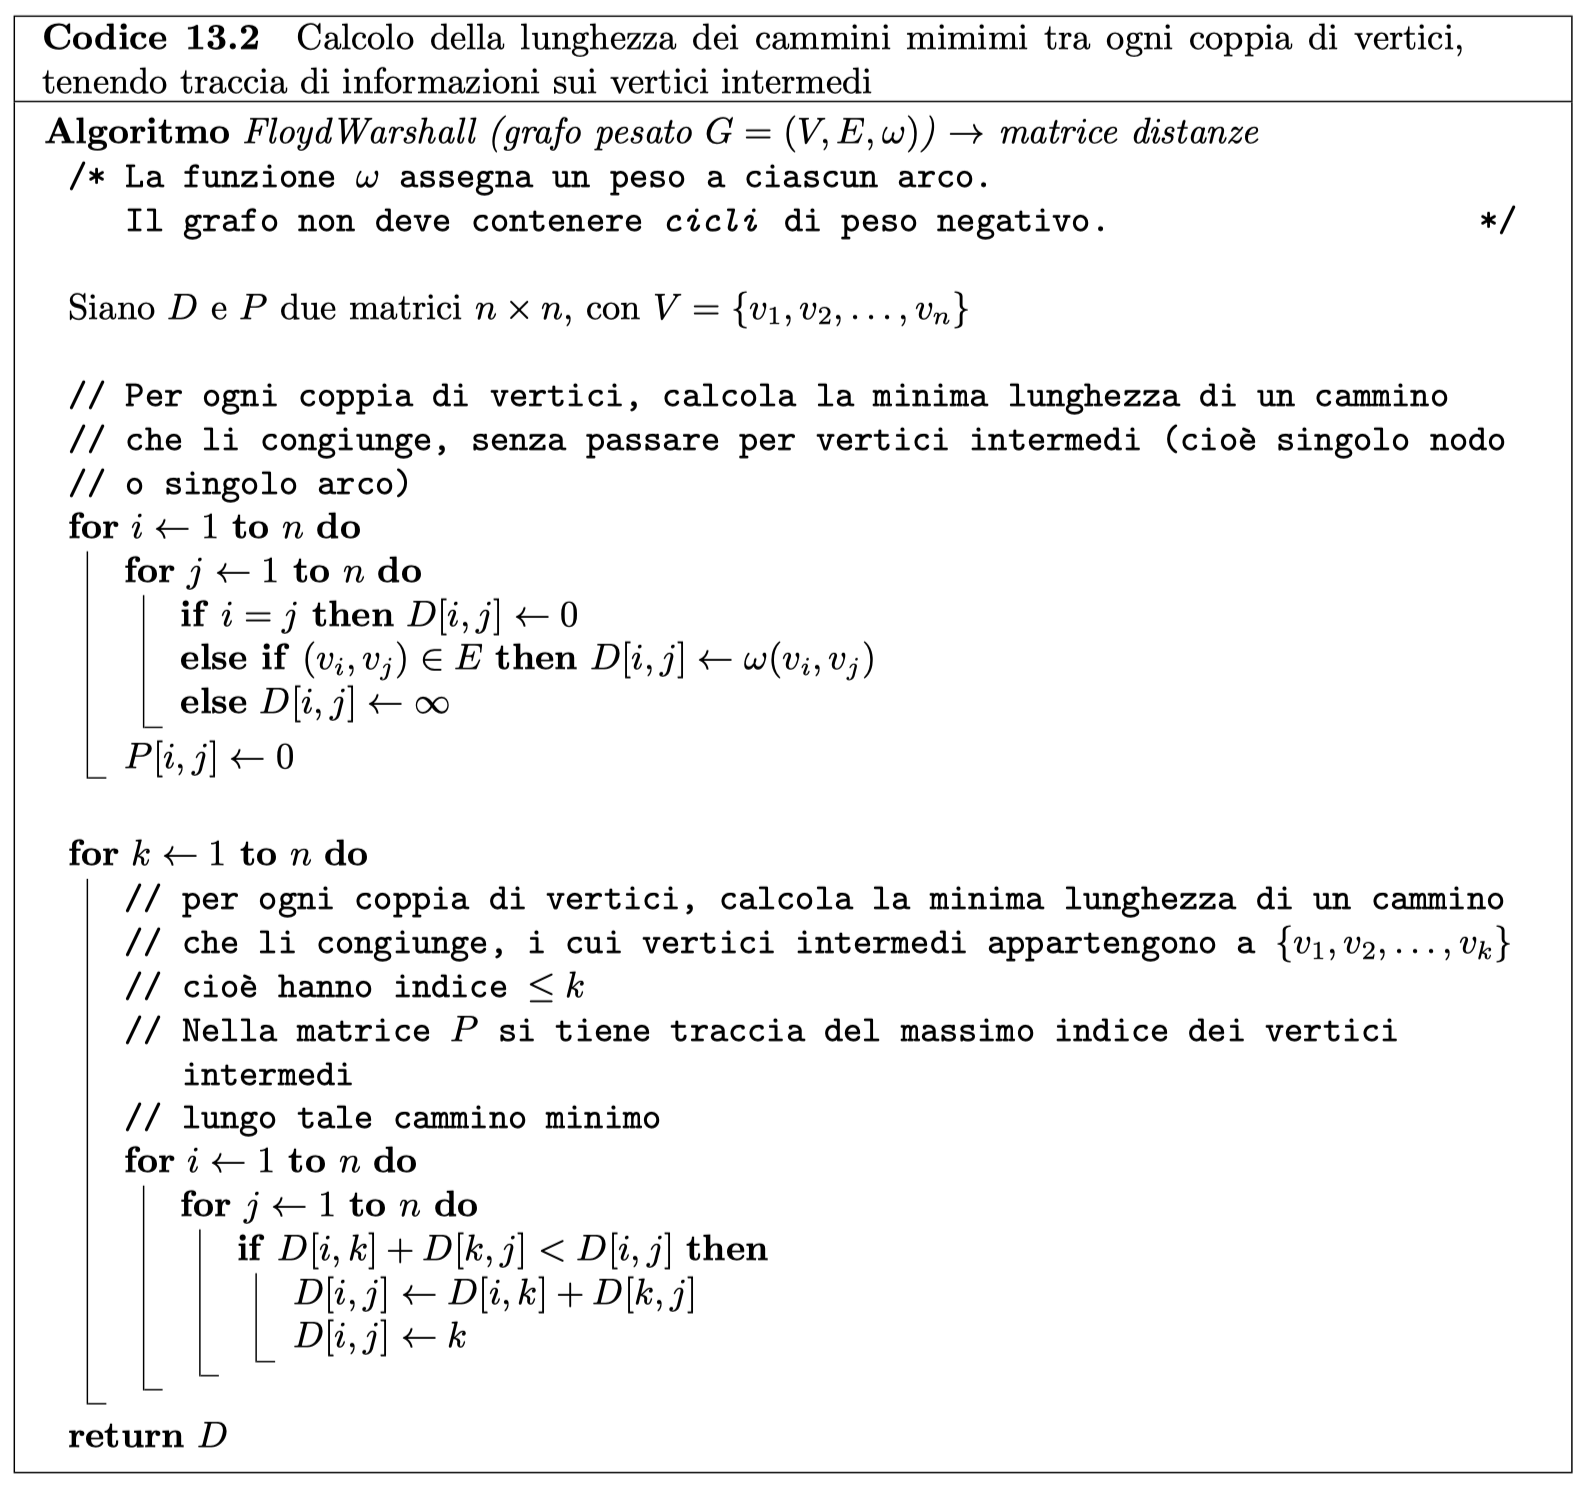
\includegraphics[width=\textwidth]{floydwarshall_2.png}
\end{figure}
\clearpage

\subsubsection{Algoritmo di Bellman e Ford}
Supponiamo di avere un grafo privo di cicli negativi.\\
\begin{itemize}
    \item $d_{v}^{[k]}$ = lunghezza del cammino minimo da $s$ a $v$ che visita al più $k$ archi.
    \item Allora la lunghezza del cammino minimo da $s$ a $v$ è $d_{v}^{[n-1]}$
    \item $d_{v}^{[0]}$ = $\begin{cases}
        0 & \text{se} \space v = s\\
        \infty & \text{altrimenti}
    \end{cases}$
    \item $d_{v}^{[k]}$ = $min(d_{v}^{[k-1]}, d_{u}^{[k-1]} + w(u, v) \space \text{t.c} \space u \in V)$\\
\end{itemize}


\begin{figure}[h]
    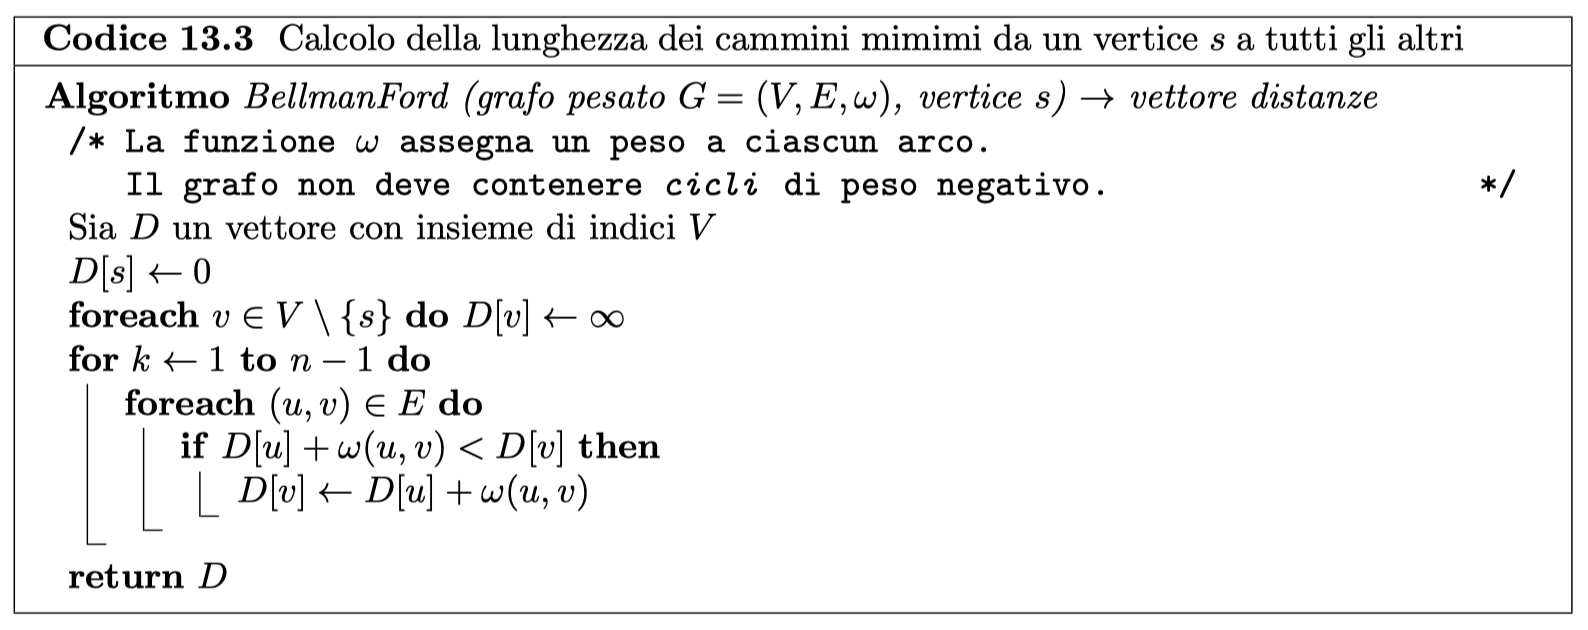
\includegraphics[width=\textwidth]{bellmanford.png}
\end{figure}

\clearpage

\subsubsection{Algoritmo di Dijsktra}
Supponiamo di avere pesi non negativi.
\begin{itemize}
    \item \textbf{Distanze provvisorie vettore $d[v]$}\\
    Inizialmente $d[v] = \begin{cases}
        0 & \text{se $v = s$}\\
        \infty & \text{altrimenti}
    \end{cases}$
    \item \textbf{$C \subseteq V$ insieme dei vertici candidati}
    Inizialmente $c = V$
    \item \textbf{Ad ogni passo strategia greedy}
    \begin{enumerate}
        \item Preleva da $C$ il vertice $u$ con $d[u]$ minima
        \item $d[u]$ diventa definitiva
        \item Aggiorna $d[v]$ per ogni $v$ adiacente a $u$
    \end{enumerate}
\end{itemize}
È implementabile utilizzando liste di adiacenza o di incidenza per rappresentare
il grafo e code con priorità.
Il tempo di esecuzione è $O(m \log n)$

\begin{figure}[h]
    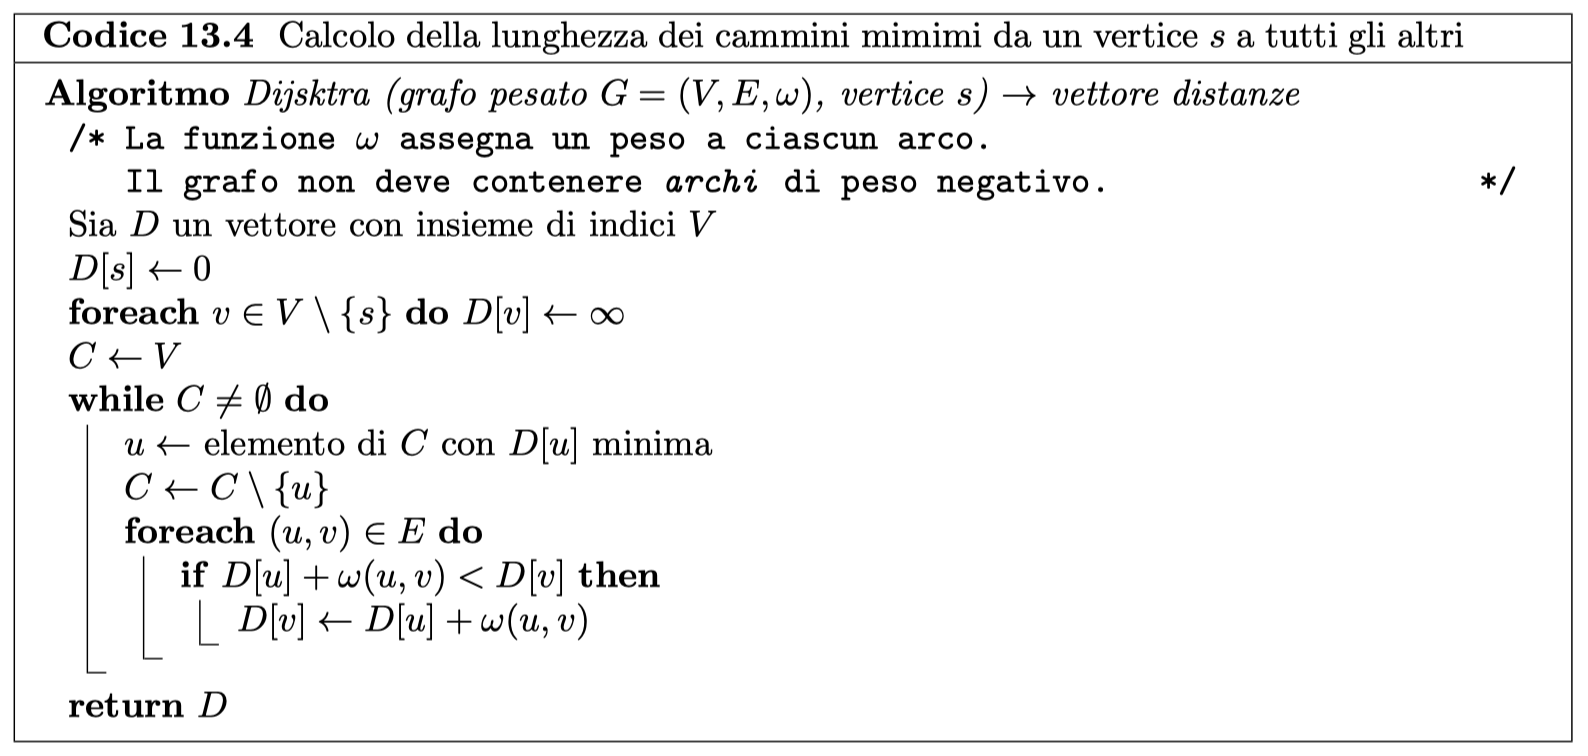
\includegraphics[width=\textwidth]{dijsktra_1.png}
\end{figure}

\begin{figure}[h]
    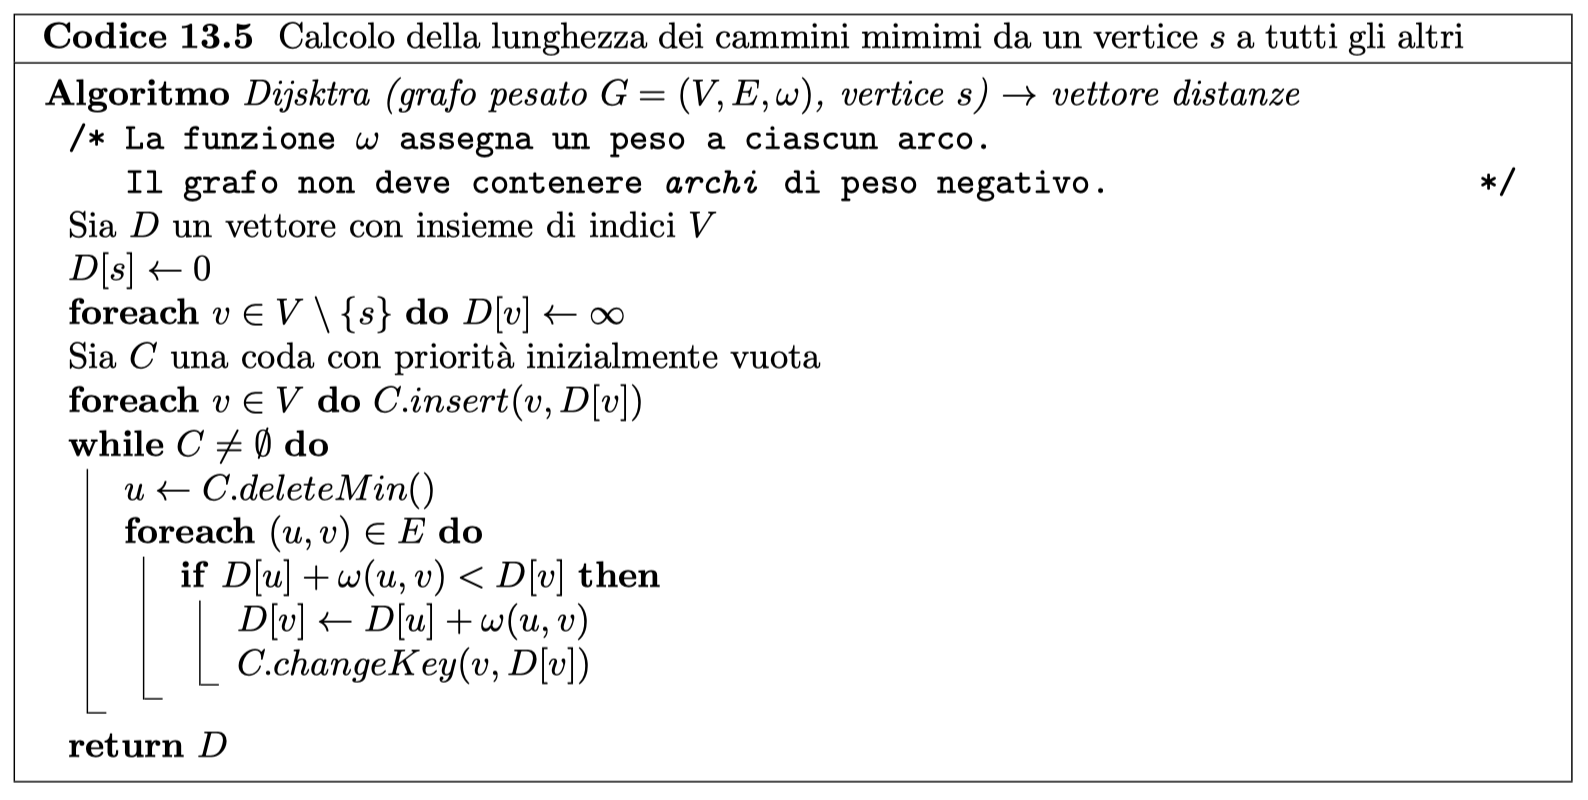
\includegraphics[width=\textwidth]{dijsktra_2.png}
\end{figure}


\clearpage